MVVM er et separerings designmønster beregnet til klient-applikationer. Meningen med mønstret er, at adskille kode der har med brugergrænsefladen at gøre, og kode der står for den underliggende logik. Mønstret er navngivet ud fra de hoveddele, det består af; model, view og viewmodel. På følgende figur ses, hvordan de tre hænger sammen:

\begin{figure}[H]
\centering
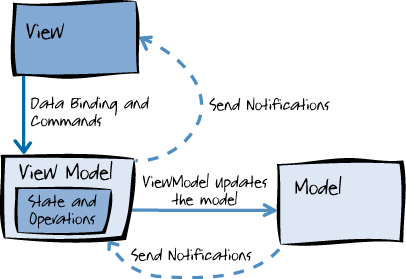
\includegraphics[width=0.6\textwidth]{Billeder/MVVM.png}
\caption{Billedet viser hvordan delene af MVVM hænger sammen.\cite{msdn1}}
\label{MVVM1}
\end{figure}

\itemize

\item \textit{Model} består af alt logikken og operationerne bag programmet og er helt uafhængigt af brugergrænsefladen. Faktisk kender \textit{model} slet ikke til \textit{view}.

\item \textit{View} er brugergrænsefladen. Det består af knapper, lister, paneler osv. Det giver brugeren den nødvendige information og registrerer brugerinput. Som følge af et brugerinput, giver \textit{View} besked til den underliggende \textit{View Model}. Det vil altså sige, at \textit{View} ikke ved, hvad der skal ske, hvis brugeren eksempelvis trykker på en given knap, men i stedet ved hjælp af commands bliver \textit{View Model} informeret og reagerer på interaktionen.  

\item \textit{View Model} er som navnet antyder bindeleddet mellem \textit{Model} og \textit{View}. \textit{View Model} får data fra \textit{Model} og formaterer disse data, sådan at \textit{View} kan præsentere dem. Herudover er meningen, at \textit{View Model} gør \textit{View} opmærksom på, om data i \textit{Model} ændres og gør på samme måde \textit{Model} opmærksom på, om data skal ændres som følge af brugerinput på \textit{View}. Hvis eksempelvis brugeren trykker på en knap, som ændrer mængden af et givet element i programmet, registreres dette af \textit{View}, som meddeler det til \textit{View Model}. \textit{View Model} kan hente den nye mængde elementer ved hjælp af data-binding mellem \textit{View} og den tilhørende \textit{View Model}-class, og opdaterer derefter \textit{Model}. Denne data-binding er to-vejs, hvilket vil sige, at \textit{View Model} også kan opdatere \textit{View} i tilfælde af ændringer i \textit{Model}.
\enditemize

Data-binding og commands, er  funktioner som WPF stiller til rådighed. Derfor udgør WPF og MVVM tilsammen en ganske stærk kombination. Data-binding kan, som tidligere nævnt, bruges som en forbindelse mellem brugerfladen og logikken. Man kan med de rette indstillinger på bindingen opnå, at når data ændres, opdateres denne ændring automatisk på de elementer, som er bundet til dataen \cite{msdn-databinding}. Denne binding er sædvanligvis to-vejs, da man som oftest ønsker at opdateringen sker begge veje. 
Meningen med commands er at adskille det objekt, der påkalder en kommando, fra logikken der eksekverer kommandoen. Dette passer godt overens med ideen bag MVVM. 

På denne måde bliver alt, der har med brugerfladen at gøre skilt fra logikken bag programmet. Disse er altså uafhængige og dette har flere fordele:

\begin{itemize}

\item {Tests kan køres på \textit{View Model} uafhængigt af \textit{View}.}
Det vil sige, at man kan teste al logikken uden at skulle igennem brugerfladen. Dette gør det langt mere fordelagtigt at skrive unit-tests, da man på den måde kan instantiere klasser uafhængigt af brugerflade.
\item{\textit{View} kan om-designes uden at resten af koden skal omskrives.}
Dette kan lade sige gøre, idet \textit{View} er skrevet udelukkende i xaml, og en ny version burde derved virke med den eksisterende \textit{View Model}.
\item{Idet brugergrænsefladen er skilt fra logikken, er udvidelse af systemet lettere.\cite{msdn1}}

\end{itemize}

